\documentclass[10pt]{beamer}
\usetheme[
%%% options passed to the outer theme
%    progressstyle=movCircCnt,   %either fixedCircCnt, movCircCnt, or corner
%    rotationcw,          % change the rotation direction from counter-clockwise to clockwise
%    shownavsym          % show the navigation symbols
  ]{AAUsimple}
  
% If you want to change the colors of the various elements in the theme, edit and uncomment the following lines
% Change the bar and sidebar colors:
%\setbeamercolor{AAUsimple}{fg=red!20,bg=red}
%\setbeamercolor{sidebar}{bg=red!20}
% Change the color of the structural elements:
%\setbeamercolor{structure}{fg=red}
% Change the frame title text color:
%\setbeamercolor{frametitle}{fg=blue}
% Change the normal text color background:
%\setbeamercolor{normal text}{fg=black,bg=gray!10}
% ... and you can of course change a lot more - see the beamer user manual.
\usepackage{pifont}
\usepackage[utf8]{inputenc}
\usepackage[english]{babel}
\usepackage[T1]{fontenc}
\usepackage{listings}
\usepackage{amsmath}
\usepackage{amssymb}
\usepackage{semantic}
\usepackage{changepage}
% Or whatever. Note that the encoding and the font should match. If T1
% does not look nice, try deleting the line with the fontenc.
\usepackage{helvet}

% colored hyperlinks
\newcommand{\chref}[2]{%
  \href{#1}{{\usebeamercolor[bg]{AAUsimple}#2}}%
}

\newcommand{\semsp}{\hspace{20px}}
\newcommand{\semnl}{\vspace{10px}}

\title{Modelling Java Bytecode}

\subtitle{Assessing Bit Flip Attacks and Countermeasures} % could also be a conference name

\date{\today}

\author[cnduru11 \and kthoms10]{
  Christoffer Nd\~ur\~u
  \href{mailto:cnuduru11@student.aau.dk}{{\tt (cnduru11)}}\\
  Kristian Mikkel Thomsen  \href{mailto:kthoms10@student.aau.dk}{{\tt (kthoms10)}}\\
}

% - Give the names in the same order as they appear in the paper.
% - Use the \inst{?} command only if the authors have different
%   affiliation. See the beamer manual for an example

\institute[
%  {\includegraphics[scale=0.2]{aau_segl}}\\ %insert a company, department or university logo
  Dept.\ of Distributed Systems\\
  Aalborg University\\
  Denmark
] % optional - is placed in the bottom of the sidebar on every slide
{% is placed on the bottom of the title page
  Department of Distributed Systems\\
  Aalborg University\\
  Denmark
  
  %there must be an empty line above this line - otherwise some unwanted space is added between the university and the country (I do not know why;( )
}

% specify a logo on the titlepage (you can specify additional logos an include them in 
% institute command below
\pgfdeclareimage[height=1.5cm]{titlepagelogo}{AAUgraphics/aau_logo_new} % placed on the title page
%\pgfdeclareimage[height=1.5cm]{titlepagelogo2}{AAUgraphics/aau_logo_new} % placed on the title page
\titlegraphic{% is placed on the bottom of the title page
  \pgfuseimage{titlepagelogo}
%  \hspace{1cm}\pgfuseimage{titlepagelogo2}
}

\begin{document}
% the titlepage
{\aauwavesbg%
\begin{frame}[plain,noframenumbering] % the plain option removes the header from the title page
  \titlepage
\end{frame}}
%%%%%%%%%%%%%%%%

% TOC
% \begin{frame}{Agenda}{}
% \tableofcontents
% \end{frame}

\section{Nduru}
% Frames

% Attack => Et attack paa det eksempel Dennis gennemgaar  (scenariet)

% Countermeasures => Vis hvordan et countermeasure kunne vaere implementeret paa det eksempel

\begin{frame}[fragile]{Bite}
Færøerne transition to smart cards for personal identification
\end{frame}

\begin{frame}[fragile]{How can faults be introduced?}
Faults can come from natural and artificial sources\\~\\
	\begin{itemize}
	\item Cosmic radiation
	\item Electric equipment
	\item Laser
	\item Infrared radiation (e.g. light bulb)\\~\\
	\end{itemize}
\end{frame}

\begin{frame}[fragile]{Field of Bit \& Instruction Differentiation}
\begin{itemize}
\item Mapping of instructions to opcodes could be changed to improve security
\item What if FoB was not implemented in the JCVM?
\end{itemize}
\end{frame}

\begin{frame}[fragile]{Field of Bit \& Instruction Differentiation}
Example
\end{frame}

\begin{frame}[fragile]{Our Solution}
\begin{figure}
\centering
\def\svgwidth{\columnwidth}
%% Creator: Inkscape inkscape 0.48.4, www.inkscape.org
%% PDF/EPS/PS + LaTeX output extension by Johan Engelen, 2010
%% Accompanies image file 'workflow_new_blank.pdf' (pdf, eps, ps)
%%
%% To include the image in your LaTeX document, write
%%   \input{<filename>.pdf_tex}
%%  instead of
%%   \includegraphics{<filename>.pdf}
%% To scale the image, write
%%   \def\svgwidth{<desired width>}
%%   \input{<filename>.pdf_tex}
%%  instead of
%%   \includegraphics[width=<desired width>]{<filename>.pdf}
%%
%% Images with a different path to the parent latex file can
%% be accessed with the `import' package (which may need to be
%% installed) using
%%   \usepackage{import}
%% in the preamble, and then including the image with
%%   \import{<path to file>}{<filename>.pdf_tex}
%% Alternatively, one can specify
%%   \graphicspath{{<path to file>/}}
%% 
%% For more information, please see info/svg-inkscape on CTAN:
%%   http://tug.ctan.org/tex-archive/info/svg-inkscape
%%
\begingroup%
  \makeatletter%
  \providecommand\color[2][]{%
    \errmessage{(Inkscape) Color is used for the text in Inkscape, but the package 'color.sty' is not loaded}%
    \renewcommand\color[2][]{}%
  }%
  \providecommand\transparent[1]{%
    \errmessage{(Inkscape) Transparency is used (non-zero) for the text in Inkscape, but the package 'transparent.sty' is not loaded}%
    \renewcommand\transparent[1]{}%
  }%
  \providecommand\rotatebox[2]{#2}%
  \ifx\svgwidth\undefined%
    \setlength{\unitlength}{361.0997458bp}%
    \ifx\svgscale\undefined%
      \relax%
    \else%
      \setlength{\unitlength}{\unitlength * \real{\svgscale}}%
    \fi%
  \else%
    \setlength{\unitlength}{\svgwidth}%
  \fi%
  \global\let\svgwidth\undefined%
  \global\let\svgscale\undefined%
  \makeatother%
  \begin{picture}(1,0.18633991)%
    \put(0,0){
\includegraphics[width=\unitlength]{figures/workflow_new_blank.pdf}}%
    \put(0.09240599,0.11){\color[rgb]{1,1,1}\hspace{-5px}\parbox[t]{0pt}{\tiny{1:} \\ \makebox(0,0)[b]{\hspace{10px}\tiny{Java bytecode}}}}%
    \put(0.23582069,0.11082579){\color[rgb]{.4,.4,1}\makebox(0,0)[lb]{\footnotesize{\textit{conversion}}}}%
    \put(0.57628484,0.11082579){\color[rgb]{.4,.4,1}\makebox(0,0)[lb]{\textit{\footnotesize{property verification}}}}%
    \put(0.49614524,0.11){\color[rgb]{1,1,1}\hspace{-5px}\parbox[t]{0pt}{\tiny{2:} \\ \makebox(0,0)[b]{\hspace{10px}\tiny{UPPAAL model}}}}%
    \put(0.90772511,0.11){\color[rgb]{1,1,1}\hspace{-5px}\parbox[t]{0pt}{\tiny{3:} \\ \makebox(0,0)[b]{\hspace{10px}\tiny{Assessment}}}}%
  \end{picture}%
\endgroup%

\caption{The workflow of the solution, from Java bytecode to UPPAAL SMC model and assessment of the modelled program.}
\label{fig:workflow_new}
\end{figure}
\end{frame}

%\begin{frame}[fragile]{Modelling Multiple Bit Flips in UPPAAL}
%\begin{itemize}
%\item Limitations of current fault model
%\subitem Semantics for describing failed reads / writes
%\item Multiple bit flips	
%\end{itemize}
%\end{frame}

\begin{frame}[fragile]{Extended Solution}
test
\end{frame}

\section{Kristian}
% Frames

% Rewriting => Giv et overview over de tools, konkret eksempel paa hvordan man implementerer det i et af tools'ene, kig paa hvilke features der er i hvert tool og stil det mere systematisk op end i rapporten

\begin{frame}{Bytecode Annotation}{}
\begin{itemize}
\item When does a fault compromise the code?
\item What is a sensitive region and how do we determine a successful run?
\item What about variable inputs? 
\end{itemize}
%\textit{figure to the left with critical region not defined}
\end{frame}
%focused security, selectiv

\begin{frame}[fragile]{Bytecode Annotation}{}
\begin{minipage}{.35\textwidth}
\begin{itemize}
\item Define variable sets
\item Selective countermeasure implementation
\item Assessments
\end{itemize}

\end{minipage}%
\hspace{10px}
\begin{minipage}{0.60\textwidth}
\begin{lstlisting}[frame=single]
public int stub()
 0: push 7  //*VALID(1,3,5)
 	          //*INVALID(2,4)
 2: ireturn 

public int foo() //*Secure
...
 4: ifeq 9
 7: aload_5 
 8: athrow
 9: aload_0  //*ASSERT VALID
...
\end{lstlisting}
\end{minipage}
\end{frame}

\begin{frame}[fragile]{UPPAAL Representation}{Virtual}


\begin{lstlisting}[frame=single]
public int foo() { return bar() + 1; }
public int bar() { return 4; }
\end{lstlisting}

\begin{figure}
\centering
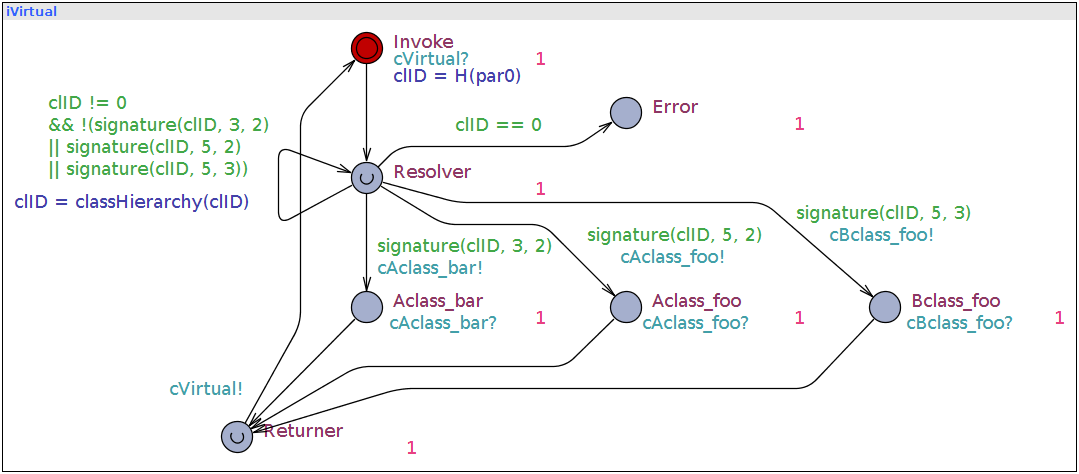
\includegraphics[width=0.8\textwidth]{figures/oldvirtual.png}
\caption{\footnotesize Virtual template as it apears in the virtual example}
\end{figure}
\end{frame}

\begin{frame}[fragile]{Representation}{Virtual}
\begin{figure}
\centering
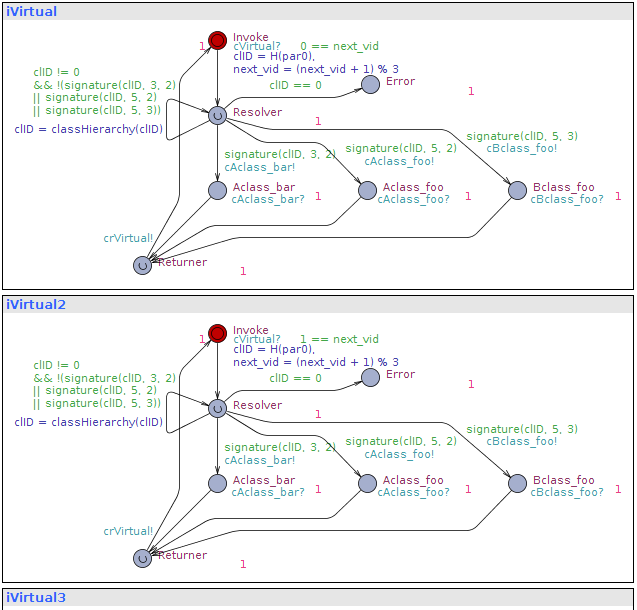
\includegraphics[width=0.6\textwidth]{figures/newVirtual.png}
\caption{\footnotesize A virtual template foreach virtual method.}
\end{figure}
\end{frame}

\begin{frame}{Representation}{}
\begin{block}{Possible solution: Single template for all methods.}
\begin{itemize}
\item Remove waiting locations.
\item Replace all channel synchronisation with edges for method calls.
\item Make a representation for the Call Stack.
\end{itemize}

\end{block}
\end{frame}


% {\aauwavesbg
% \begin{frame}[plain,noframenumbering]
%   \finalpage{Questions?}
% \end{frame}}
%%%%%%%%%%%%%%%%

\end{document}

%%% Local Variables:
%%% mode: latex
%%% TeX-master: "AAUsimpletheme"
%%% End:
